\documentclass[11pt]{article}
\usepackage[utf8]{inputenc}
\usepackage[english]{babel}
\usepackage{amsfonts, amsmath, amssymb}
\usepackage{graphicx}
\usepackage[height=8.5in, width=11in, margin=1in]{geometry}
\usepackage{titling}
\usepackage{float}
\usepackage{caption}
\usepackage{setspace}
\usepackage{booktabs}
\usepackage{tabularx}
\usepackage{fancyhdr}
\usepackage[hidelinks]{hyperref}
\usepackage[all]{hypcap}
\usepackage{caption}
\usepackage[nottoc,numbib]{tocbibind}
\usepackage{pgfgantt}

\title{Exoni Final Design Report}
\author{Egor Gorelyy, Taim Al-Dabbagh, Hasan Khan, Nolen Zhao}
\date{May 2023}

\begin{document}

\pagenumbering{roman}
\newgeometry{width=11in,top=2in}
\begin{titlingpage}
    \centering

    {\huge\bfseries Exoni Final Design Report\par}\vspace{18pt}
    
\includegraphics[]{figures/uwlogo.PNG}\par
    {\LARGE \textbf{Department of Mechanical and Mechatronics Engineering}\par}\vspace{2cm}

    {\large \textbf{A Report Prepared For:}\par}\vspace{2pt}
    {\large Professor Andrew Morton\par}\vspace{2pt}
    {\large Professor Baris Fidan\par}\vspace{24pt}

    {\large \textbf{Authors:}\par}\vspace{2pt}
    {\large Egor Gorelyy, 20953858 \par}\vspace{2pt}
    {\large Taim Al-Dabbagh, 20964898 \par}\vspace{2pt}
    {\large Hasan Khan, 20928382 \par}\vspace{2pt}
    {\large Nolen Zhao, 20932971 \par}\vspace{2pt}
    {\large 200 University Ave W. \par}\vspace{2pt}
    {\large Waterloo, Ontario, N2L 3G1 \par}\vspace{2pt}
    \vspace{36pt}

    {\large April 6, 2026\par}\vspace{4pt}
    \vfill

\end{titlingpage}
\restoregeometry \setstretch{1.5}
\pagenumbering{arabic}

\tableofcontents
\newpage

% --- 1. INTRODUCTION (20%) ---
\section{Introduction}

\subsection{Background}
Exoni is an open-source powered knee exoskeleton designed for outdoor recreational use. The system targets mobility-limited users who wish to maintain their hiking and running intensity — functioning analogously to an e-bike, but for lower-limb assistance. Unlike clinical rehabilitation exoskeletons, which are designed for indoor, low-speed, supervised environments, an outdoor exoskeleton must operate across variable terrain, tolerate ambient temperature variation, and remain safe and comfortable for extended wear. This imposes a distinct set of engineering constraints: the device must maximize power density within a small form factor, dissipate heat passively while remaining cool to the touch, and remain transparent to the user's natural gait when unpowered (backdrivable).

The core actuation challenge stems from the human knee joint, which requires peak torques on the order of 0.5 - 1 Nm/kg during stair climbing and loaded hiking. For a representative user mass, this drives a gearbox output torque requirement of approximately 20 Nm (or around 40\% of knee torque). Achieving this with a motor small enough to mount at the knee joint, light enough to avoid gait disruption, and cool enough to maintain skin-contact safety requires a custom motor design — off-the-shelf motors at this power level are either too large, too heavy, or thermally unviable for wearable use.

In order to power the exoskeleton, including the motor, an electrical system needs to exist. Off-the-shelf boards do not exist that meet requirements such as reading from multiple IMUs, running FOC control on the motor, sending telemetry data wirelessly, and more. Therefore, the electrical system requires the use of custom PCBs (printed circuit board) that are designed to meet the requirements in order to have a working knee exoskeleton. Equally, the firmware running on those boards must meet real-time constraints that no off-the-shelf embedded framework satisfies out of the box: the motor drive loop must execute at 1~kHz to maintain stable FOC commutation, the current-sense ADCs must be calibrated and synchronized with the PWM carrier, and the encoder must be read and decoded within the same tick. This necessitated a custom firmware architecture built on FreeRTOS, with a dedicated high-priority task for motor control and a separate task for the outer impedance control loop.

\subsection{Needs Assessment \& Problem Formulation}
% TODO: Expand with user research, clinical need framing, and market context from MTE 481 report.

The target user population is individuals with mild-to-moderate lower limb weakness or fatigue --- including older adults, post-injury patients in later-stage rehabilitation, or able-bodied users under high load conditions such as multi-day backpacking. The core unmet need is a portable, lightweight powered knee assist device that does not compromise natural movement when unpowered.

The problem can be formally stated as: design and build a powered knee exoskeleton with an integrated custom motor and drivetrain that meets the constraints specified in Section~\ref{sec:constraints}, with particular emphasis on the conflicting demands of high torque output, low backdrive resistance, passive thermal safety, and minimal mass.

\subsection{Constraints and Criteria}
\label{sec:constraints}

The design constraints were derived from biomechanical requirements, user comfort considerations, and practical fabrication limitations. Table~\ref{tab:constraints} summarizes the key mechanical constraints and their target values, and Table~\ref{tab:fw_constraints} summarizes the key firmware and control constraints.

\begin{table}[H]
\centering
\caption{Mechanical Design Constraints and Targets}
\label{tab:constraints}
\begin{tabular}{ll}
\toprule
\textbf{Constraint} & \textbf{Target} \\
\midrule
Outer motor diameter & $<$ 100~mm \\
Gearbox output torque & 17.6~Nm \\
Backdrive torque & $<$ 1~Nm \\
Surface temperature & $\leq$ 43~\textdegree{}C \\
Motor weight & 600~g \\
Full system weight & 1.5~kg \\
\bottomrule
\end{tabular}
\end{table}

\begin{table}[H]
\centering
\caption{Firmware and Control Constraints and Targets}
\label{tab:fw_constraints}
\begin{tabular}{ll}
\toprule
\textbf{Constraint} & \textbf{Target} \\
\midrule
FOC inner loop rate & 1~kHz \\
Outer impedance loop rate & 200~Hz \\
PWM switching frequency & 20~kHz \\
Current sense resolution & 12-bit ADC \\
Encoder resolution & 14-bit ($\leq 0.022^\circ$/count) \\
Phase overcurrent trip threshold & 15~A \\
Telemetry latency & $\leq$ 5~ms (binary frame at 200~Hz) \\
\bottomrule
\end{tabular}
\end{table}

The 1 Nm requirement for backdrive torque is a limit for a system to feel backdrivable to a human. 43C is the maximum temperature that still feels comfortable. These constraints directly conflict. Higher output torque requires higher current draw, which increases both heat generation (scaling as $I^2 R$) and cogging torque (increasing backdrive resistance). Reducing mass reduces the thermal mass available for heat storage and the cross-sectional area available for conduction paths. These tradeoffs cannot be resolved by intuition alone: simulation was required to inform both the electromagnetic and thermal design of the motor and battery pack.

\subsection{Design Review}
% TODO: Summarize the MTE 481 design selection process --- morphological charts, concept screening, Pugh matrices, etc.
% The following summarizes the high-level architecture selection rationale informed by the simulation-driven design approach.

The design pipeline proceeded through five sequential stages, each feeding quantitative results forward to the next:

\begin{enumerate}
    \item \textbf{Electromagnetic analysis:} Ansys Maxwell simulations were used to select the stator frame (7210 vs.\ 8110) and rotor magnetic configuration (iron-backed, ironless, and multiple Halbach array geometries) based on torque constant ($K_t$, in Nm/A) and motor constant ($K_m$, in Nm/$\sqrt{\text{W}}$), the latter being the relevant figure of merit for a thermally constrained motor.

    \item \textbf{Motor thermal analysis:} SimScale conjugate heat transfer (CHT) simulations assessed whether passive cooling could maintain surface temperatures below 43~\textdegree{}C under the electromagnetic loss inputs from Stage 1. Iterative geometry modifications were evaluated.

    \item \textbf{Battery thermal analysis:} SimScale CHT simulations evaluated the effect of battery pack configuration (series vs.\ parallel cell arrangement) and housing geometry on cell surface temperatures, with a 35~\textdegree{}C safety limit.

    \item \textbf{Firmware and control design:} A custom FreeRTOS firmware was developed for the STM32G474, implementing a 1~kHz Field Oriented Control (FOC) inner loop and a 200~Hz impedance control outer loop. Key decisions included the dual-task scheduling architecture, the SVPWM modulation strategy with third-harmonic injection, and the encoder electrical angle alignment procedure. PI current controller gains were tuned analytically and verified against the live telemetry stream.

    \item \textbf{Final design:} Outputs from all four stages were consolidated into the final hardware and software specification.

\end{enumerate}


% --- 2. FINAL DESIGN (35%) ---
\section{Final Design}

\subsection{Final Design Details}

\subsubsection{Halbach Array BLDC Motor Design}

\paragraph{Stator Selection}

The electromagnetic design began with a selection between two commercially available stator frames: the 7210 frame (72~mm diameter, 36 slots, 7 turns per tooth) and the 8110 frame (81~mm diameter, 24 slots, 13 turns per tooth). Ansys Maxwell's analytical equation solver was used to compute the motor constants for each configuration, with wire turns per slot limited by the physical copper fill factor of each slot geometry.

The relevant figure of merit for a thermally constrained wearable motor is the motor constant $K_m = K_t / \sqrt{R}$ (in Nm/$\sqrt{\text{W}}$), which quantifies torque output per unit of heat generated. Although the 7210 frame yields an 11\% higher torque constant ($K_t = 0.124$~Nm/A vs.\ $0.112$~Nm/A for the 8110), its higher phase resistance means it produces 23\% more heat for the same torque --- a motor constant of 0.399 vs.\ 0.444 for the 8110. Accordingly, the \textbf{8110 frame} was selected as the basis for the motor design.

Model verification used the analytical relationship $K_t \propto N_\text{phase} \times d_\text{stator}$, where $N_\text{phase}$ is the total turns per phase. The predicted relative torque constants ($7210: 13 \times 8 \times 72 = 7488$; $8110: 7 \times 12 \times 81 = 6804$) were consistent with the simulated values, confirming the model.
\begin{figure}
    \centering
    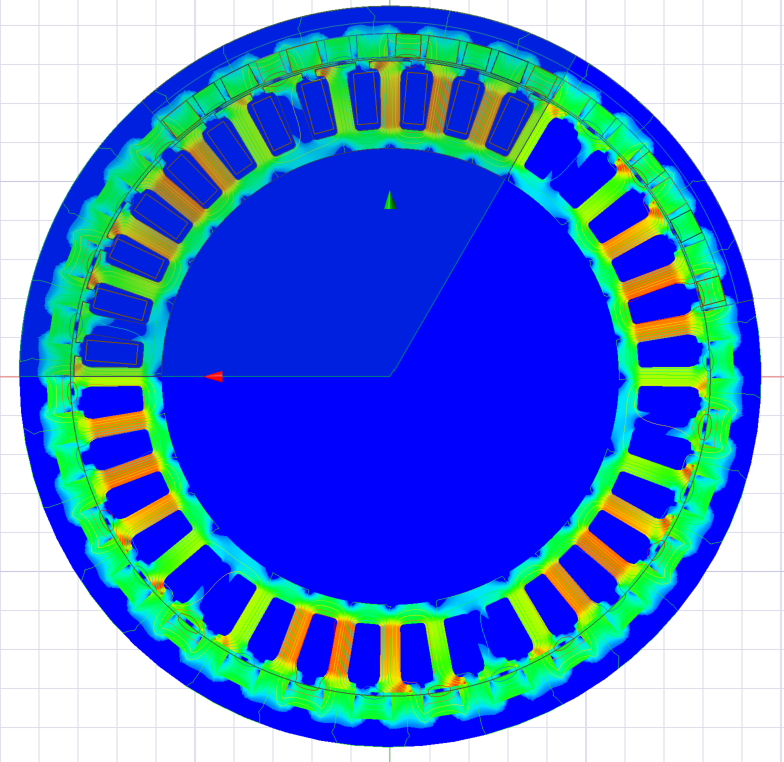
\includegraphics[width=0.5\linewidth]{figures/stator.png}
    \caption{ANSYS Electromagnetic Stator and Rotor Simulation}
    \label{fig:stator_sim}
\end{figure}
\begin{table}[H]
\centering
\caption{Stator Sizing Simulation Results}
\label{tab:stator}
\begin{tabular}{lll}
\toprule
 & \textbf{7210 Frame} & \textbf{8110 Frame} \\
\midrule
Diameter & 72~mm & 81~mm \\
Slots & 36 & 24 \\
Turns per tooth & 7 & 13 \\
Torque Constant $K_t$ (Nm/A) & 0.124 & 0.112 \\
Motor Constant $K_m$ (Nm/$\sqrt{\text{W}}$) & 0.399 & \textbf{0.444} \\
\bottomrule
\end{tabular}
\end{table}

\paragraph{Rotor Configuration}

Having fixed the stator, the rotor magnetic configuration was selected to optimise the tradeoff between torque constant ($K_t$) and backdrivability (quantified by peak cogging torque). Five configurations were evaluated using 2D Ansys Maxwell transient motor simulations: iron-backed, ironless, and three Halbach array geometries with varying main and auxiliary magnet dimensions. Input data comprised measured magnet dimensions and datasheet performance characteristics (remanence, coercivity).

The key assumption underpinning the backdrivability analysis is that gearbox friction is minimised through the 8.4:1 planetary gearbox design, making backdrive resistance predominantly a function of magnetic cogging torque rather than mechanical friction.

Halbach arrays concentrate magnetic flux on the airgap-facing side of the rotor by varying magnet orientation, eliminating the need for a heavy steel back-iron yoke. This simultaneously reduces rotor mass and, by reducing the flux linkage variation with rotor angle that drives cogging, lowers peak cogging torque. Table~\ref{tab:rotor} summarises simulation results.
\begin{figure}
    \centering
    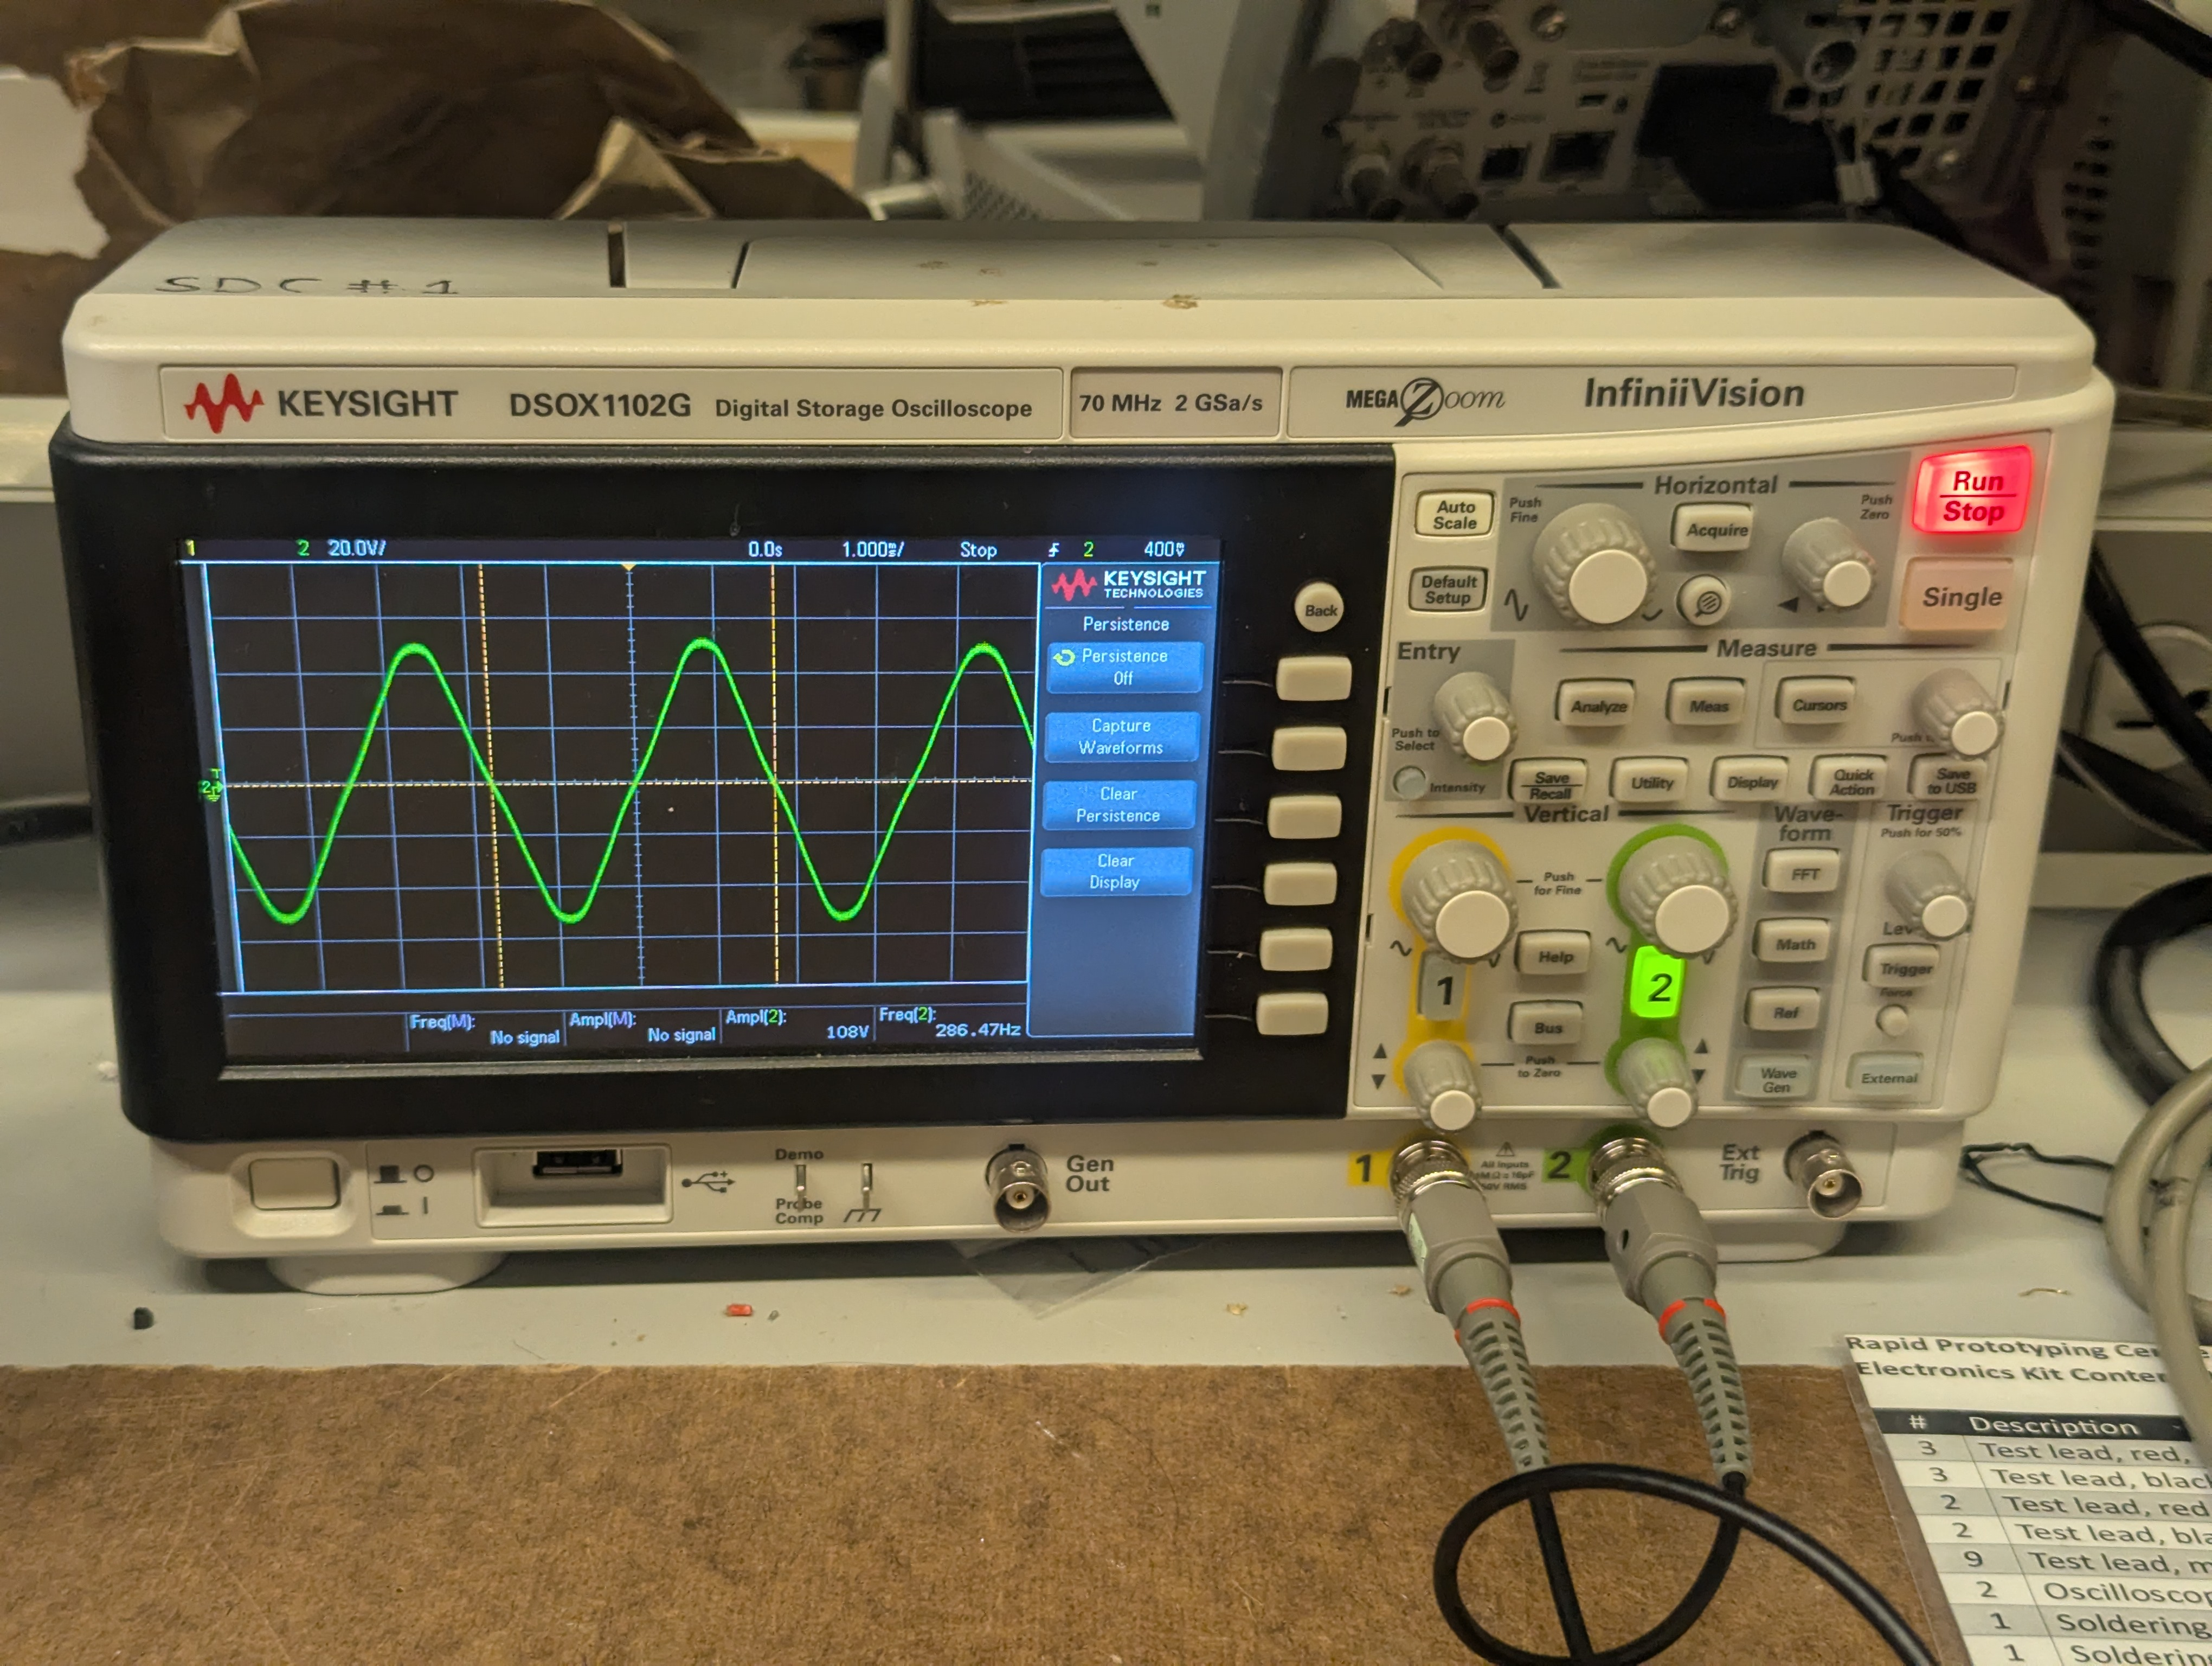
\includegraphics[width=0.5\linewidth]{figures/emf.jpg}
    \caption{Back EMF Measurement for Testing Purposes}
    \label{fig:back_emf}
\end{figure}
\begin{table}[H]
\centering
\caption{Rotor Configuration Simulation Results}
\label{tab:rotor}
\begin{tabular}{lll}
\toprule
\textbf{Arrangement} & \textbf{$K_t$ (Nm/A)} & \textbf{Peak Cogging Torque (Nm)} \\
\midrule
Iron-backed & 0.118 & 0.166 \\
Ironless & 0.097 & 0.137 \\
Halbach (4~mm, 1.6~mm) & 0.103 & 0.010 \\
\textbf{Halbach (4~mm, 3.2~mm)} & \textbf{0.110} & \textbf{0.011} \\
Halbach (3~mm, 2~mm) & 0.098 & 0.012 \\
\bottomrule
\end{tabular}
\end{table}

The \textbf{Halbach (4~mm, 3.2~mm)} configuration was selected: it achieves the highest $K_t$ among Halbach variants (0.110~Nm/A) while reducing peak cogging torque by approximately $15\times$ relative to the iron-backed baseline. The resulting aluminum rotor weighs 44~g versus 127~g for a comparable steel rotor --- a 2.88$\times$ mass reduction.

\paragraph{Simulation Verification}

Cogging torque was verified by measuring the torque required to manually rotate the physical motor across one electrical cycle. The measured peak cogging torque of 0.02~Nm is in close agreement with the simulated 0.011~Nm, confirming that the Halbach configuration meets the $<$1~Nm backdrive target by a large margin. Harmonic analysis (FFT) of the measured cogging waveform shows dominant components at the 36th harmonic (corresponding to 36 stator slots) and the 30th harmonic (corresponding to 30 rotor poles), consistent with the known slot-pole combination.
\begin{figure}
    \centering
    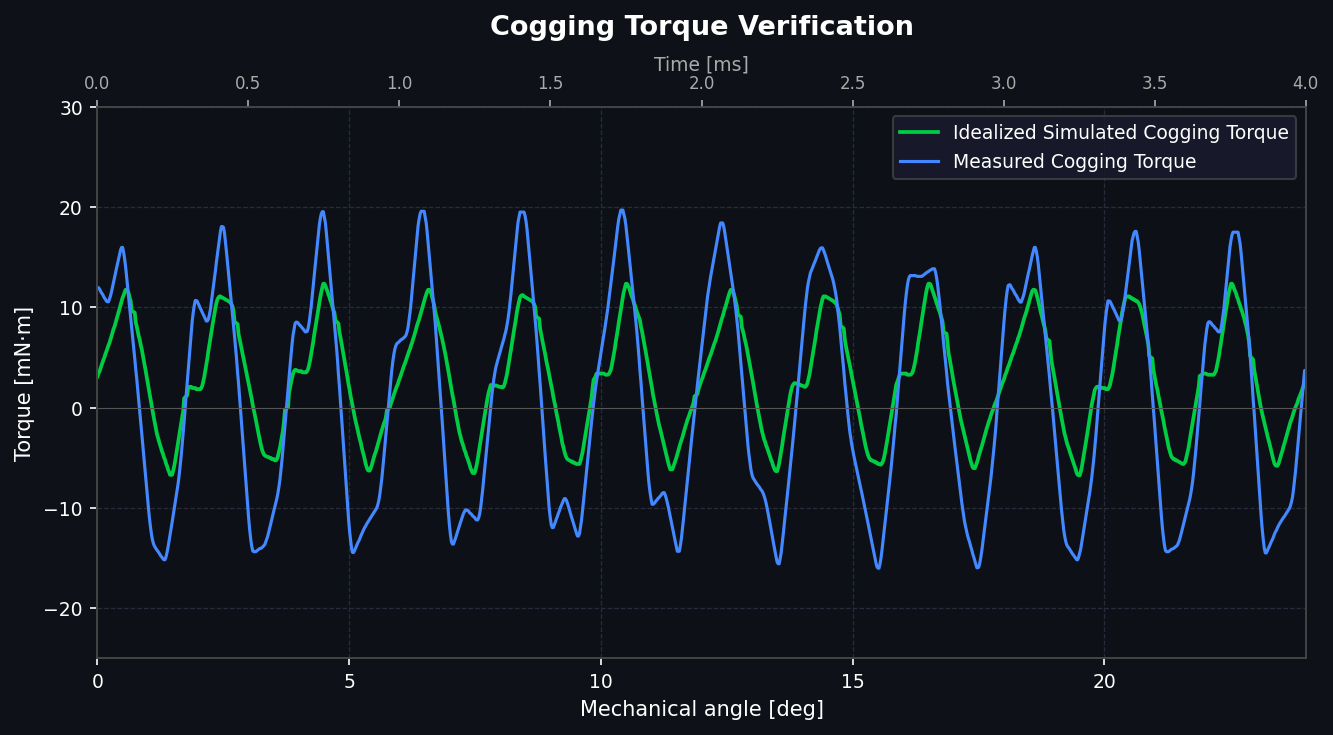
\includegraphics[width=0.5\linewidth]{cogging torque.png}
    \caption{Cogging Torque Verification}
    \label{fig:cogging_torque}
\end{figure}
Torque constant was verified via back-EMF measurement on the physical prototype. The first motor iteration yielded $K_t$ 22\% below simulation, attributed to 2D simulation limitations (inability to capture axial flux fringing and end-turn effects) and manufacturing tolerances in magnet placement. Following design refinements in the second iteration, measured $K_t$ was within 5\% of simulation. Table~\ref{tab:rotor_impact} summarises the cumulative improvement from the electromagnetic analysis.

\begin{table}[H]
\centering
\caption{Impact of Rotor Configuration Analysis on Final Design}
\label{tab:rotor_impact}
\begin{tabular}{llll}
\toprule
\textbf{Metric} & \textbf{Iron-Backed Default} & \textbf{With Analysis} & \textbf{Improvement} \\
\midrule
Measured Torque Constant & 0.67 & 0.97 & 1.45$\times$ \\
Rotor Weight & 127~g (steel) & 44~g (aluminum) & 2.88$\times$ \\
Backdrive Torque & 1.6~Nm & 0.26~Nm & $6\times$ \\
Motor Constant & 0.26 & 0.31 & 19\% \\
$K_t$ Agreement with Simulation & 78\% & 94\% & +16\% \\
\bottomrule
\end{tabular}
\end{table}

\subsubsection{Electrical Subsystem}
% TODO: Detail the custom PCB, cable routing/management, and custom 8S Li-ion battery pack design.

A block diagram was first done to architect the electrical system, as shown in Figure \ref{fig:electricalSystemOverview} below. 3 unique PCBAs (Printed Circuit Board Assembly) were designed.

    \begin{figure}[H]
        \centering
        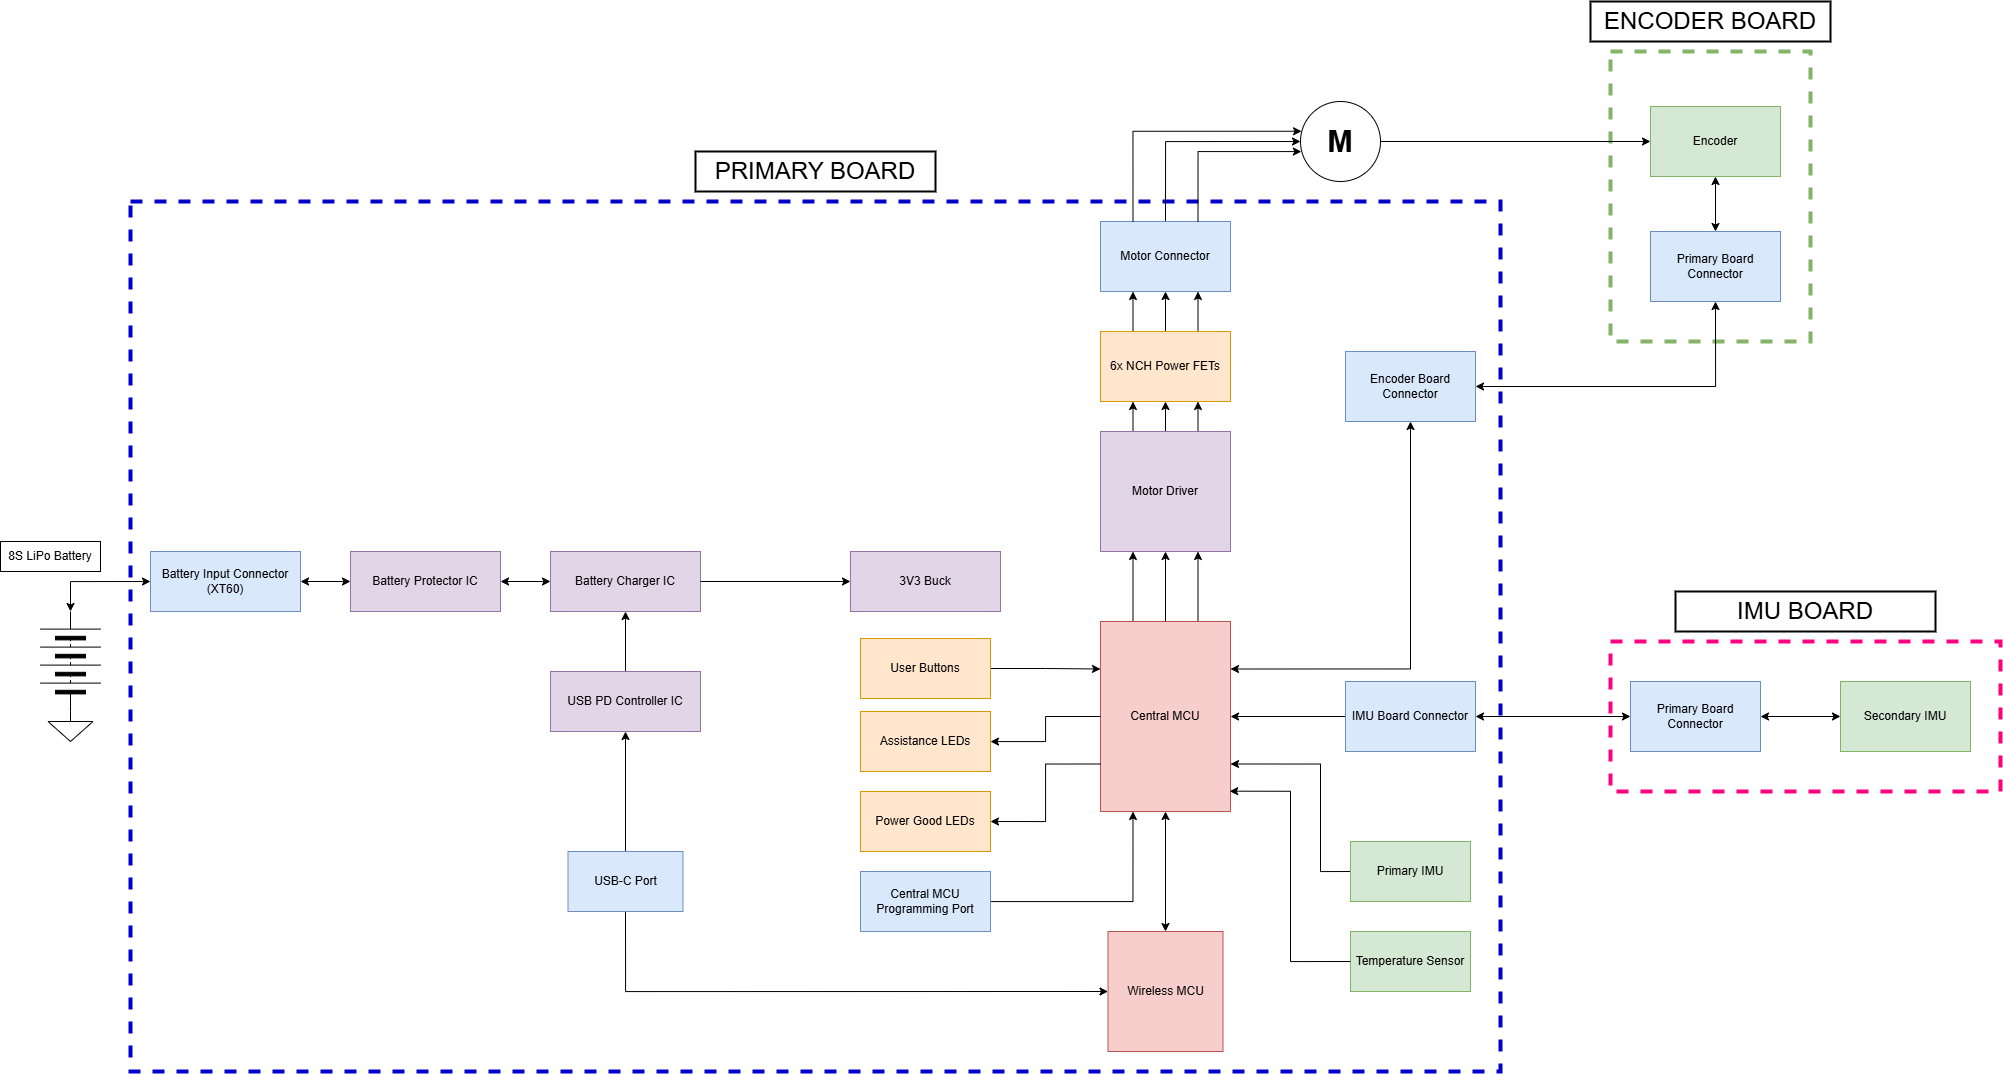
\includegraphics[width=1\linewidth]{figures/electricalSystemOverview.png}
        \caption{Electrical System Overview}
        \label{fig:electricalSystemOverview}
    \end{figure}
    \begin{itemize}
        \item \textbf{Primary Board:} The main board that contains bulk of the exoskeleton's functionality. The board features a BMS (which is composed of a battery monitoring and battery charger IC). The battery charger IC also has power path management, which is important for the USB-C input. USB-PD is used to negotiate more power from the USB-C input's respective source. The BMS automatically handles power path switching, deciding whether the battery or USB-C powers the entire low-voltage system. The low-voltage system composes of two micro-controllers, an STM32G474 and ESP32-S3-MINI-1. The STM32 handles the bulk of the work, where it inferences from the model, reads from the sensors over SPI, and drives the custom motor. The ESP32 deals with the BMS, transmits wireless data, enables OTA, and handles other low-critcal tasks.
        \item \textbf{Encoder Board:} The encoder board is a board placed by the custom motor, to read encoder/position data which is fed back to the priamry board through a custom shielded JST-XH cable. The encoder data is used for FOC motor control.
        \item \textbf{IMU Board:} The IMU board is a small board that only has a IMU, the same one featured in the primary board. This allows to have a IMU by the lower half of the user's leg, which is used to calculate knee angles and have the model recognize the user's gait cycle. It is also connected to the primary board through a custom shielded JST-XH cable.
    \end{itemize}

    All 3 PCBAs were designed using KiCad, an open-source EDA (electronic design automation) tool. The boards were manufactured and assembled by JLCPCB in China. 3D views of the primary, encoder, and IMU board are shown below in Figures \ref{fig:3DPrimary}, \ref{fig:3DEncoder}, and \ref{fig:3DIMU} respectively.

    \begin{figure}[H]
        \centering
        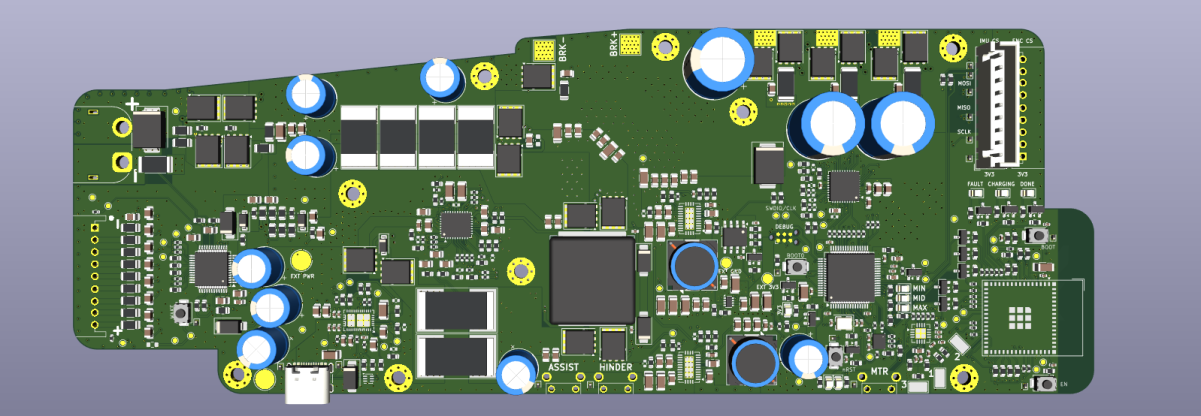
\includegraphics[width=1\linewidth]{figures/primaryBoard3D.png}
        \caption{3D View of Primary Board}
        \label{fig:3DPrimary}
    \end{figure}

    \begin{figure}[H]
        \centering
        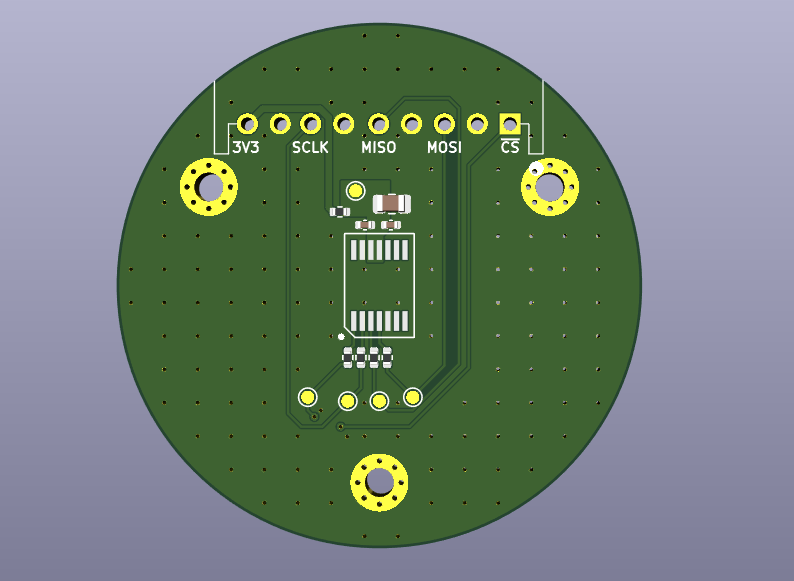
\includegraphics[width=0.8\linewidth]{figures/encoderBoard3D.png}
        \caption{3D View of Encoder Board}
        \label{fig:3DEncoder}
    \end{figure}

    \begin{figure}[H]
        \centering
        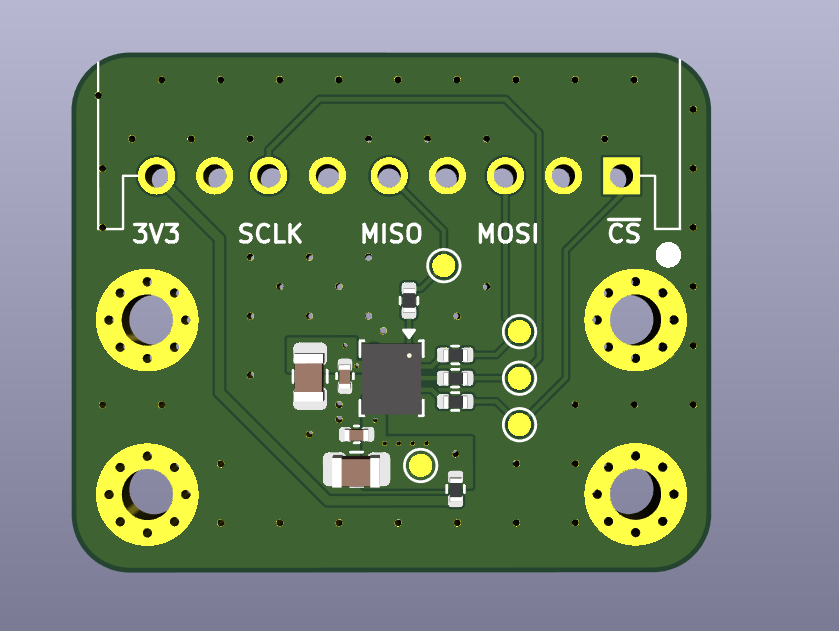
\includegraphics[width=0.8\linewidth]{figures/imuBoard3D.png}
        \caption{3D View of IMU Board}
        \label{fig:3DIMU}
    \end{figure}

\subsubsection{Firmware and Software}
\label{sec:firmware}

The STM32G474 firmware is written in C and runs under FreeRTOS 10.3.1 with a 1~kHz scheduler tick. Two tasks divide the real-time workload: a high-priority sensor/motor task running at 1~kHz and a normal-priority control task running at 200~Hz.

\paragraph{FreeRTOS Task Architecture}

\textbf{StartDefaultTask} executes at 1~kHz and is the highest-priority task on the system. Each iteration reads the AS5048A magnetic encoder via SPI, converts the 14-bit raw count to a mechanical angle (rad), and computes the electrical angle by scaling by the motor's pole-pair count. Every fifth iteration (200~Hz), it reads both LSM6DSVETR IMUs and writes their accelerometer and gyroscope snapshots to volatile shared buffers, then issues an \texttt{xTaskNotifyGive} to wake the ControlTask. On each 1~kHz tick it calls \texttt{Motor\_Step}, which advances the FOC commutation loop and writes new PWM duty cycles to TIM1. The task also monitors the DRV8323 fault pin (\texttt{MTR\_nFAULT}): if a fault is detected it disables the motor enable line and retries every 500~ms. Two telemetry streams are produced: a human-readable CSV log at 100~Hz over UART2 to the ESP32, and a compact 43-byte binary frame at 200~Hz containing encoder angle, both IMU readings, the current torque command, and a CRC-8 integrity check.

\textbf{ControlTask} runs at 200~Hz and is woken exclusively by \texttt{xTaskNotifyTake}, ensuring it executes only when fresh IMU data is available. It reads the latest IMU and encoder snapshots, computes knee angular velocity via finite difference, applies an impedance control law to produce a torque command, converts that torque to a q-axis current reference, and writes the result to a shared volatile variable consumed by the FOC loop.

\paragraph{Field Oriented Control}

FOC decouples the motor's torque-producing and flux-producing current components, enabling precise torque control by regulating two DC quantities (the d- and q-axis currents) rather than three sinusoidal phase currents. The control loop executes at 1~kHz inside \texttt{Motor\_Step}.

Phase currents are measured on two of the three motor phases using 1~m$\Omega$ shunt resistors and the DRV8323's integrated current-sense amplifiers at a gain of 20~V/V. The DRV8323 is a gate driver and current-sense amplifier IC from Texas Instruments, selected for its integrated three-phase gate driver, adjustable current-sense gain, and hardware over-current protection. Outputs are digitised by ADC3 and ADC4 on the STM32, each running at 12-bit resolution with 47.5-cycle sampling. Current offset calibration (\texttt{FOC\_CalibrateOffsets}) averages 64 ADC readings at zero current to remove amplifier bias from all subsequent measurements.

The Clarke transform converts the two measured phase currents $i_a$ and $i_b$ to the stationary $\alpha$-$\beta$ frame, exploiting Kirchhoff's current law ($i_c = -(i_a + i_b)$):
\begin{align}
    i_\alpha &= i_a \\
    i_\beta  &= \frac{i_a + 2i_b}{\sqrt{3}}
\end{align}

The Park transform then rotates the stationary frame into the rotor-synchronous $d$-$q$ frame using the electrical angle $\theta_e$:
\begin{align}
    i_d &=  i_\alpha \cos\theta_e + i_\beta \sin\theta_e \\
    i_q &= -i_\alpha \sin\theta_e + i_\beta \cos\theta_e
\end{align}

Two independent PI controllers close the loop on $i_d$ and $i_q$ separately, each running at 1~kHz with a timestep of $\Delta t = 1$~ms and anti-windup integrator clamping. For torque control the d-axis reference is held at zero (no flux weakening) and the q-axis reference is set by the outer impedance loop. The PI gains used for the custom 15-pole-pair motor are $K_{p,d} = 0.3$, $K_{i,d} = 1.0$, $K_{p,q} = 1.0$, $K_{i,q} = 100.0$, with output limits of $\pm$24~V corresponding to the half-bus voltage. An over-current trip at 15~A per phase immediately zeros all PWM outputs and resets the PI integrators.

The PI voltage outputs are transformed back to the stationary frame via the inverse Park transform, then converted to three-phase duty cycles using Space Vector PWM (SVPWM) with third-harmonic common-mode injection. Common-mode injection extends the linear modulation range to approximately 15\% beyond sine-triangle PWM for the same DC bus voltage:
\begin{equation}
    v_\text{cm} = -\frac{\max(v_a, v_b, v_c) + \min(v_a, v_b, v_c)}{2}
\end{equation}
The resulting duty cycles are written to TIM1's capture/compare registers. TIM1 is configured in centre-aligned mode at 20~kHz (ARR = 399 at 16~MHz) with 500~ns of dead time on each complementary output pair to prevent shoot-through in the three half-bridge legs of the DRV8323.

\paragraph{Encoder and Angle Calibration}

The AS5048A is a 14-bit magnetic rotary encoder read over SPI at Mode 1 (CPOL = 0, CPHA = 1) using a pipelined read protocol: each transaction issues the angle register address (0x3FFF) and simultaneously receives the result of the previous request, reducing latency by one SPI frame. The 14-bit raw count spans 0--16383 counts per revolution (0.022$^\circ$/count, $3.84 \times 10^{-4}$~rad/count).

Before closed-loop operation, an electrical angle alignment routine maps the encoder frame to the motor's electrical frame. The STM32 applies a fixed d-axis voltage at electrical angle $\theta_e = -\pi/2$ for one second, locking the rotor to Phase~A's magnetic zero. The encoder angle at this position, scaled by the pole-pair count, gives the electrical offset $\theta_\text{offset}$ that is subtracted from all subsequent angle computations:
\begin{equation}
    \theta_e = \theta_\text{mech} \times P_p - \theta_\text{offset}
\end{equation}

\paragraph{Motor Control Modes and Soft-Start}

The firmware supports four motor control modes managed by \texttt{motor\_cntrl.c}: \texttt{MOTOR\_MODE\_OFF} (PWM zeroed), \texttt{MOTOR\_MODE\_OPEN\_LOOP} (fixed $V_q$ with internal angle ramp, independent of encoder), \texttt{MOTOR\_MODE\_CLOSED\_LOOP} (FOC with PI current control at a fixed $I_q$ reference), and \texttt{MOTOR\_MODE\_IMPEDANCE} (outer impedance loop sets $I_q$). At startup, the system enters open-loop mode and ramps the q-axis voltage linearly from 0 to 3.0~V over 200~ms to limit inrush current and allow the motor to establish rotation before encoder-based commutation takes over.

\paragraph{Impedance Control Outer Loop}

The 200~Hz ControlTask implements a virtual impedance law that converts a desired joint stiffness and damping into a q-axis current command:
\begin{equation}
    I_q = K(\theta_\text{des} - \theta) - D\,\dot{\theta}
\end{equation}
where $K$ is the virtual stiffness (A/rad), $D$ is the virtual damping (A$\cdot$s/rad), $\theta$ is the measured knee angle, and $\dot{\theta}$ is the finite-difference angular velocity estimate. The current command is passed to the FOC inner loop, which regulates the physical phase currents to track it. Converting $I_q$ to output torque uses the motor torque constant and gearbox ratio: $\tau_\text{output} = K_t \cdot I_q \cdot N_\text{gear}$, where $K_t = 0.110$~Nm/A and $N_\text{gear} = 8.4$.

\paragraph{Telemetry}

The STM32 streams two data formats over UART2 at 921600~baud to the ESP32-S3. A 43-byte binary frame transmitted at 200~Hz contains synchronisation bytes, a sequence counter, encoder angle in centidegrees, six-axis IMU data from both sensors (accelerometer in units of $10^{-4}$~m/s$^2$, gyroscope in units of $10^{-3}$~deg/s), knee angular velocity, torque command, q-axis current command, and a CRC-8 integrity byte. A human-readable CSV stream at 100~Hz logs electrical angle, phase currents, PI outputs, raw ADC counts, calibration offsets, and the fault pin state for offline debugging. The ESP32 forwards this data wirelessly and supports OTA firmware updates over Wi-Fi, decoupling the real-time STM32 loop from all wireless communication latency.

\subsection{Modifications and Deviations from Original Design}
% TODO: What changed from the MTE 481 report and why?

\subsection{Construction and Manufacturing}
\subsubsection{Mechanical Fabrication}
% TODO: Machining, 3D printing, motor assembly (magnet placement for Halbach array).

\subsubsection{Electrical Assembly}
% TODO: Spot welding the 8S battery pack, PCB assembly/soldering, cable crimping.
For the PCBAs, the soldering and assembly work was already done by JLCPCB. However, the primary board has exposed copper on the back, and if placed against a conductive material, the board will short. The reason for having copper exposed was for thermal management purposes. Having the copper exposed allows for a low thermal impedance path, as driving the motor with the 6 MOSFETs (which form the 3 half bridges, one half bridge for each motor phase) will create heat depending on how much current runs through them. With the exposed copper, the mechanical frame will act as a heat spreader and keep the primary board within a tolerable temperature range.

To prevent the board from shorting, a TIM (thermal interface material) was used between the primary board's backside and the mechanical frame it is mounted onto. The TIM pad is electrically insulating, but thermally conductive. Sheets of TIM were cut around have the same outline as the board, which both the TIM and primary board are mounted through screws to fasten to the mechanical assembly.

Aside from the PCBAs, two battery packs were made. Using the 21700 Molicell Li-Ion cells, custom 3D-printed battery pack case, and a spot welder, 8S1P battery packs were made in-house. An XT-60 cable and 9-pin JST-XH cable were soldered onto nickel strips, which the strips were used spot weld against the cells to put cells together in series. The cables come out from the 3D-printed case, which can finally connect into the primary board's input connectors for both power input and balancing input for the BMS. Figure \ref{fig:batteryPackAssembly} shows the assembly of one 8S1P battery pack, with nickel strips being spot welded onto the cells that are contained within the 3D-printed case.

    \begin{figure}[H]
        \centering
        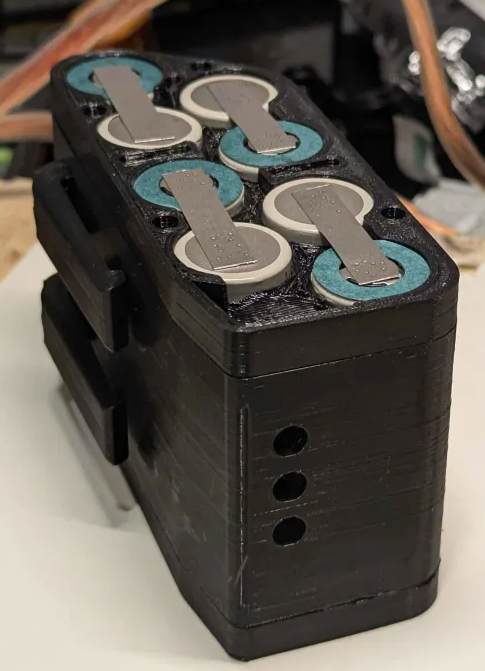
\includegraphics[width=0.5\linewidth]{figures/batteryPackAssembly.png}
        \caption{Assembly of 8S1P Li-Ion battery pack}
        \label{fig:batteryPackAssembly}
    \end{figure}

\subsection{Commissioning (Component Functional Tests)}
\subsubsection{Motor Bring-up \& Testing}
% TODO: No-load tests, phase resistance checks, back-EMF measurement procedure.

\subsubsection{PCB \& Battery Bring-up}
% TODO: Voltage checks, continuity, BMS testing on the 8S pack.
All 3 PCBAs (primary, encoder, and IMU) were inspected visually and tested. Inspection was done to look for quality of soldering, if potential issues exist like a short, cracks within components, and so forth. A digital multimeter was used for continuity testing to verify no shorts exist. After checking no clear problem exists, a USB-C was plugged in. Later on, a problem with turn-on time with the BMS was found after trying to plug in the board with a USB-C coming from a different laptop where power was switching on and off. This was fixed by adding additional capacitance on the gate-source of the back-to-back high-side N-Channel MOSFETs to slow down the turn-on time. After coming across small bugs and modifications on the board to overcome such bugs, the primary board was verified to work with a functioning BMS, USB-PD IC, STM32/ESP32, and sensors. The power-path management and switchover between battery and USB-C was verified to work well, along with charging the battery through USB-C.

The battery was verified through the assembly of it. The balancing connector was used to check the voltage between each cell to verify the cells are being correctly spot welded together in the right order. The primary board was able to be powered by the custom 8S1P battery pack.

The encoder board and IMU board were brought up simply, although a shorting issue was discovered within the IMU board. This was fixed by sanding down and getting rid of the power vias (that was shorted to ground vias) by a dremel. Both boards were connected to the primary board, which code was uploaded to get data from both the encoder and second IMU which worked. All of the aforementioned tests verified the bring-up of the electrical system, which composed of the custom PCBAs, custom battery pack, and the custom cables.

\subsubsection{Firmware Flashing \& Telemetry Check}
\label{sec:fw_commissioning}

Firmware was compiled using the STM32CubeIDE toolchain (GCC ARM) and flashed to the STM32G474RE via SWD (Serial Wire Debug) using an ST-Link V3 programmer integrated on the primary board. After each flash, the UART2 CSV telemetry stream was monitored at 921600~baud using a serial terminal to confirm that sensor reads were live and values were sensible before proceeding to motor tests.

The first commissioning step was ADC current offset calibration. With the motor unpowered and all PWM outputs disabled, \texttt{FOC\_CalibrateOffsets} was called to average 64 ADC samples on both current-sense channels and store the zero-current offsets. The resulting offsets were printed over UART and inspected to confirm they fell within the expected mid-rail range of the DRV8323 current-sense amplifiers.

The encoder was verified by manually rotating the motor shaft and confirming that the reported mechanical angle in the telemetry stream increased and decreased monotonically over a full revolution, and that the 14-bit count wrapped cleanly at 0/16383. The AS5048A diagnostic register was also read to confirm the OCF (offset compensation finished) bit was set, indicating the internal offset compensation algorithm had converged.

The electrical angle alignment routine was then executed to calibrate the offset between the encoder frame and the motor's electrical frame. With the motor stationary and suspended (no load), the STM32 applied a fixed d-axis voltage for one second to lock the rotor to Phase~A's magnetic zero. The resulting \texttt{theta\_offset} value was stored and validated by stepping the motor through one open-loop electrical revolution and confirming that the commutation produced smooth rotation without vibration or stalling.

Open-loop spin-up was tested next. The motor was commanded into open-loop mode with the q-axis voltage ramp active, and the telemetry stream was used to observe the soft-start ramp reaching 3.0~V over 200~ms with no phase overcurrent trips. The motor accelerated smoothly to the open-loop target speed, confirming that the SVPWM output, dead-time insertion, and DRV8323 gate drive were all functioning correctly.

Closed-loop FOC commissioning was performed by switching to \texttt{MOTOR\_MODE\_CLOSED\_LOOP} at a low $I_q$ reference (0.5~A) and monitoring the d- and q-axis currents in the telemetry CSV. Correct closed-loop operation was confirmed when $i_d$ converged to near zero and $i_q$ tracked the reference with low steady-state error, indicating proper encoder-to-electrical-frame alignment and well-tuned PI gains. The DRV8323 fault pin state (\texttt{nfault} column in the CSV) remained high throughout, confirming no gate driver faults were triggered.

\subsection{Testing and Performance}

\paragraph{Motor Thermal Performance}

The motor thermal simulation used SimScale's conjugate heat transfer (CHT) solver, which simultaneously models conduction through the stator and housing, natural and forced internal convection, external forced convection (modelled at walking speed), and radiation from the outer housing surface. Heat inputs were drawn from the prior electromagnetic simulation: 5~W of hysteresis and eddy current losses, and 17~W of resistive ($I^2R$) winding losses at rated current draw. A bulk winding thermal conductivity of 0.5~W/m$\cdot$K was used --- significantly below that of pure copper, to account for air gaps between wires and epoxy-fill variations.

The baseline simulation predicted a surface temperature of 81~\textdegree{}C, well above the 43~\textdegree{}C target. Three sequential geometry modifications were applied and re-simulated:

\begin{table}[H]
\centering
\caption{Motor Thermal Simulation Iterations}
\label{tab:motor_thermal}
\begin{tabular}{ll}
\toprule
\textbf{Iteration} & \textbf{Predicted Surface Temperature (\textdegree{}C)} \\
\midrule
Baseline & 81 \\
1) Anodize housing (maximize radiation) & 71 \\
2) Increase external surface area (+17\%) & 63 \\
3) Thicken stator conduction path (+50\%) & 58 \\
\bottomrule
\end{tabular}
\end{table}

The simulation is intentionally conservative --- ambient airflow was modelled at walking speed (the minimum expected operating condition), and the housing was assumed sealed. As a contingency, the housing design includes provision to mill ventilation slots for forced external airflow if required in the worst case.

Experimental verification was performed by cycling the physical motor under a sinusoidal torque load and logging surface temperature via an integrated thermocouple probe. With fan airflow approximating walking speed, the housing reached a peak of 35~\textdegree{}C --- meeting specification. Under zero airflow (worst case), the housing exceeded 50~\textdegree{}C, within 15\% of the simulation prediction of 58~\textdegree{}C, validating the model fidelity. Table~\ref{tab:motor_thermal_impact} summarises the design changes driven by the thermal analysis.

\begin{table}[H]
\centering
\caption{Impact of Motor Thermal Analysis on Final Design}
\label{tab:motor_thermal_impact}
\begin{tabular}{llll}
\toprule
\textbf{Parameter} & \textbf{Without Analysis} & \textbf{With Analysis} & \textbf{Improvement} \\
\midrule
Housing finish & Bare aluminum & Anodized & $-$10~\textdegree{}C \\
Surface area & Baseline & $+$17\% & $-$8~\textdegree{}C \\
Stator cross-section & 2~mm & $+$50\% thickness & $-$5~\textdegree{}C \\
Temperature monitoring & None & Integrated probe & Live monitoring \\
\bottomrule
\end{tabular}
\end{table}
\begin{figure}
    \centering
    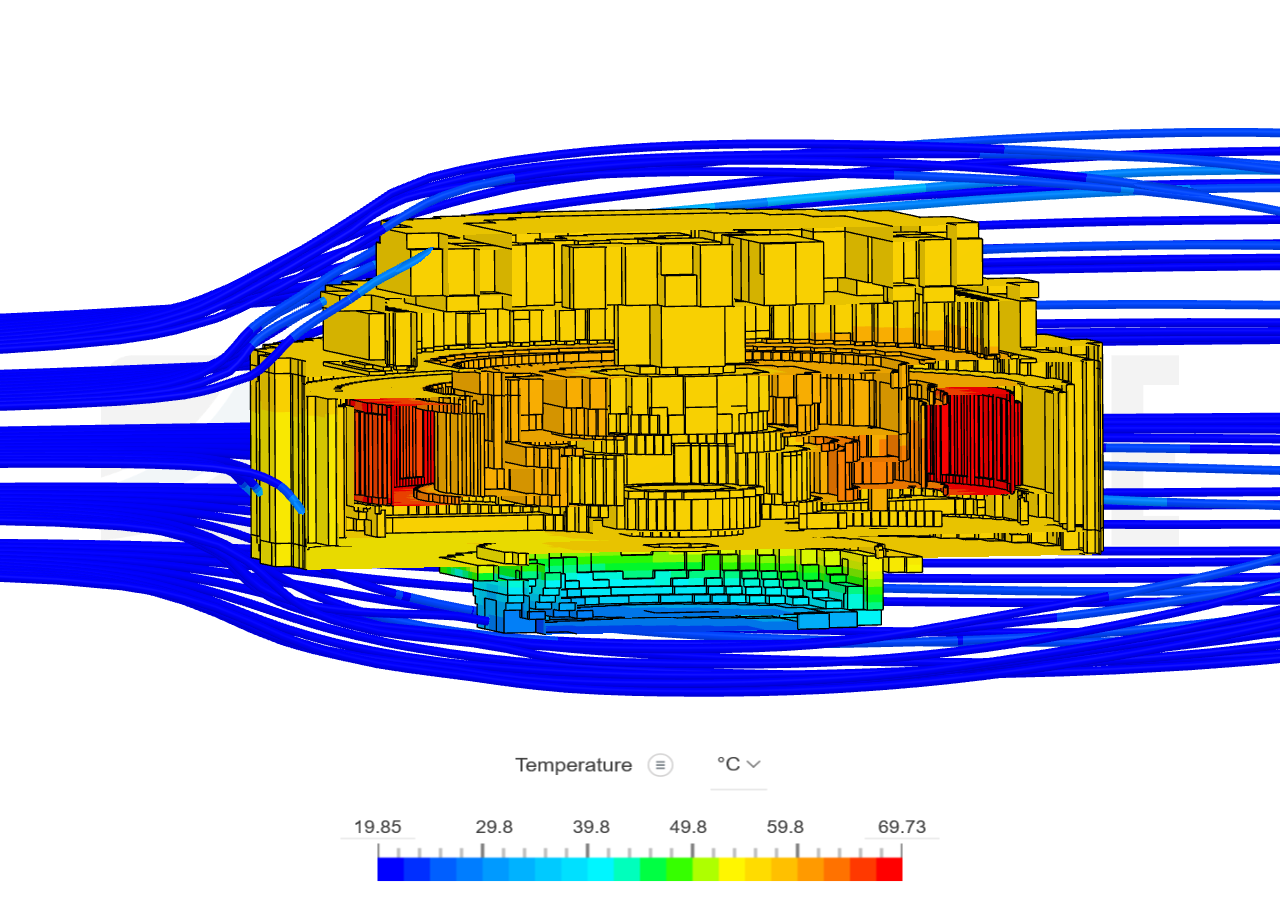
\includegraphics[width=0.5\linewidth]{figures/thermal flow.png}
    \caption{Motor Conjugate Heat Transfer Simulation}
    \label{fig:motor_cht}
\end{figure}
\begin{figure}
    \centering
    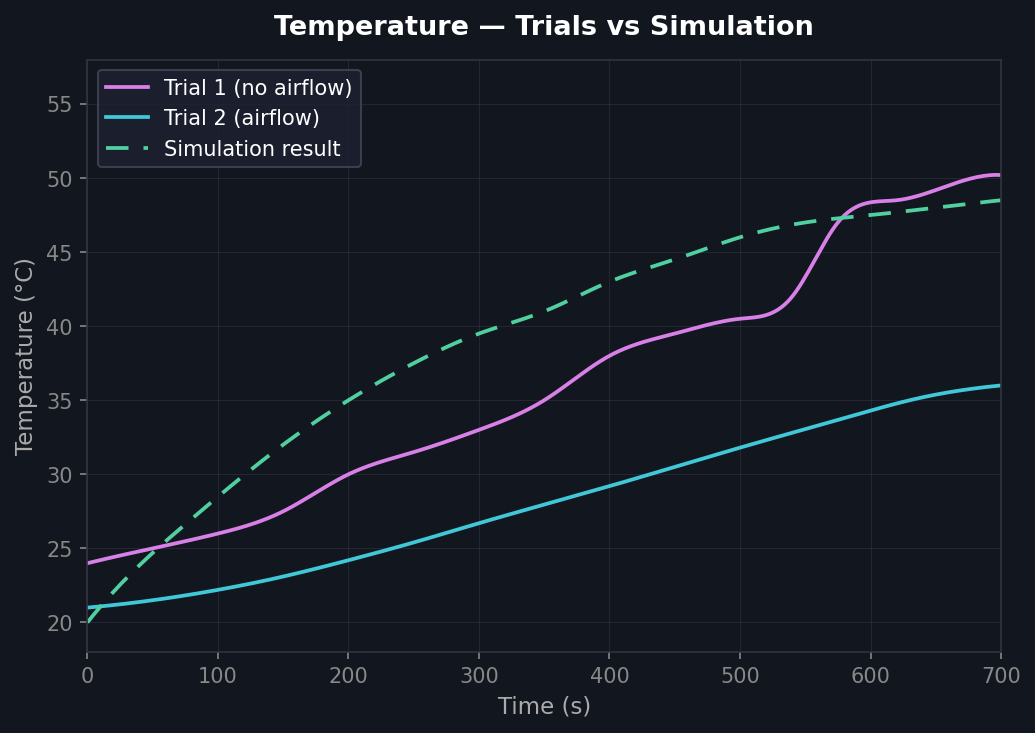
\includegraphics[width=0.5\linewidth]{figures/temp plot.png}
    \caption{Thermal Testing Data}
    \label{fig:thermal_test}
\end{figure}

\paragraph{Battery Thermal Performance}

The battery pack is mounted at the user's hip and must remain below 35~\textdegree{}C. The primary design variable was the cell configuration: more cells in parallel reduces per-cell current and thus $I^2R$ losses, but increases weight. Numerical analysis of relative heat losses across configurations (4s2p, 5s2p, 6s2p, 7s2p, 8s1p) using Molicel P45B 21700 cell internal resistance and nickel strip interconnect resistance showed that the 8s1p configuration has the highest relative heat loss per cell but the lowest total cell count and weight. The 8s1p case was therefore simulated as the worst case.

The SimScale CHT model included anisotropic cell thermal conductivity (35~W/m$\cdot$K axially, 1~W/m$\cdot$K radially) to reflect the strongly directional heat conduction of cylindrical cells. Two housing variants were compared: solid-walled and ventilated (with slots on the front face). Side-face ventilation holes were found to have no meaningful effect on cell temperatures, as the stagnation zone is primarily on the front surface facing the direction of motion. Front ventilation holes reduced cell temperatures from 35~\textdegree{}C to 26~\textdegree{}C. Housing material conductivity (PETG vs.\ expensive high-conductivity filament) had no significant effect on cell temperature, indicating conduction through the housing is not the limiting thermal resistance.

These results were cross-validated against third-party P45B characterisation data showing cell surface temperatures of approximately 40~\textdegree{}C under 30--50~A pulsed discharge --- our pack operates at lower duty cycle and peak current, making the simulated 26~\textdegree{}C plausible. Table~\ref{tab:battery_thermal_impact} summarises the design decisions driven by the battery thermal analysis.

\begin{table}[H]
\centering
\caption{Impact of Battery Thermal Analysis on Final Design}
\label{tab:battery_thermal_impact}
\begin{tabular}{llll}
\toprule
\textbf{Parameter} & \textbf{Without Analysis} & \textbf{With Analysis} & \textbf{Improvement} \\
\midrule
Configuration & 6s2p & 8s1p & $\approx$300~g saved; 4 fewer cells \\
Housing & Solid & Strategic ventilation holes & $-$10~\textdegree{}C cell temperature \\
Material & High-conductivity filament & PETG & Cost and complexity reduced \\
\bottomrule
\end{tabular}
\end{table}

\paragraph{Overall System Performance}

Table~\ref{tab:results} compares the final measured performance against the design targets from Section~\ref{sec:constraints}. All constraints were met.

\begin{table}[H]
\centering
\caption{Final Design Performance vs. Targets}
\label{tab:results}
\begin{tabular}{lll}
\toprule
\textbf{Constraint} & \textbf{Target} & \textbf{Final Design} \\
\midrule
Outer motor diameter & $<$ 100~mm & 91~mm \\
Gearbox output torque & 17.6~Nm & 20~Nm \\
Backdrive torque & $<$ 1~Nm & 0.260~Nm \\
Surface temperature & 43~\textdegree{}C & 35~\textdegree{}C \\
Motor weight & 600~g & 582~g \\
Full system weight & 1.5~kg & 1.5~kg \\
\bottomrule
\end{tabular}
\end{table}
\begin{figure}
    \centering
    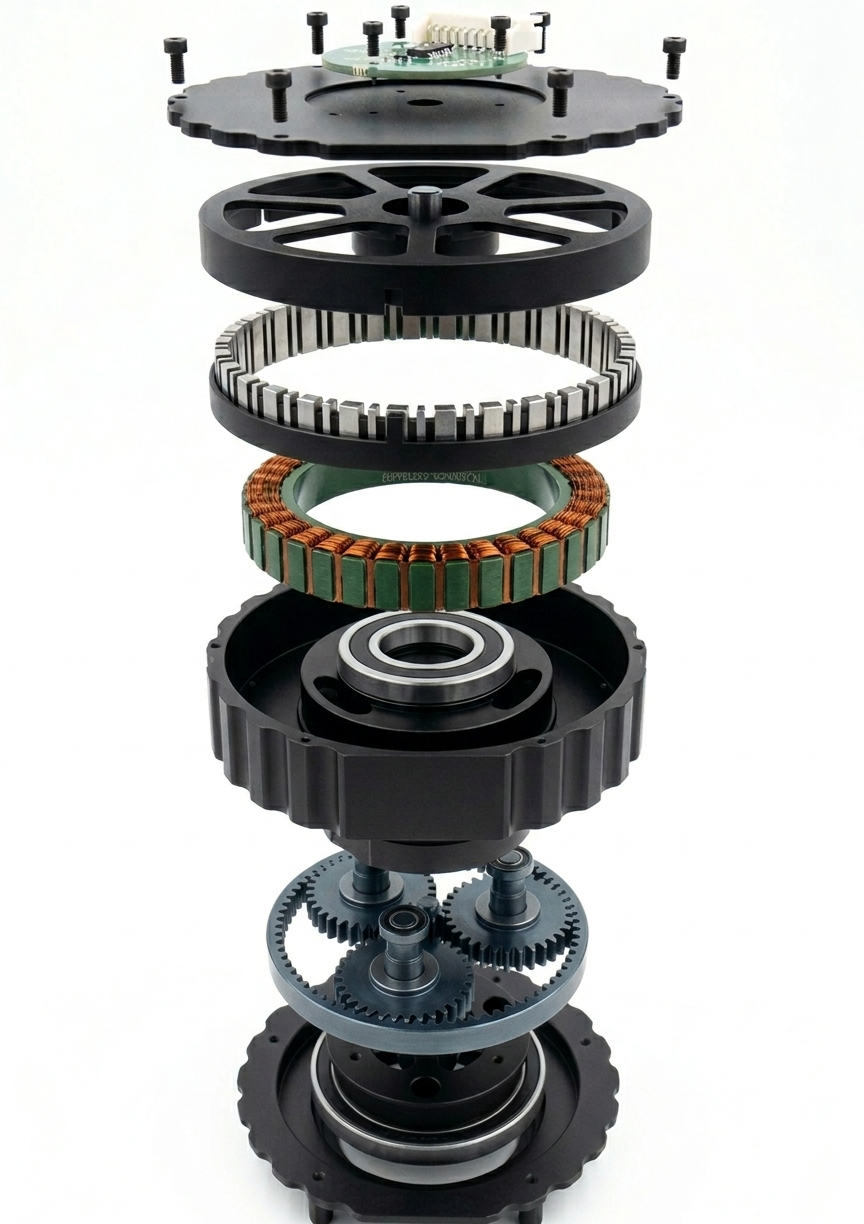
\includegraphics[width=0.5\linewidth]{figures/qdd blown up.png}
    \caption{Blown Up Motor Housing}
    \label{fig:motor_housing_exploded}
\end{figure}
\begin{figure}
    \centering
    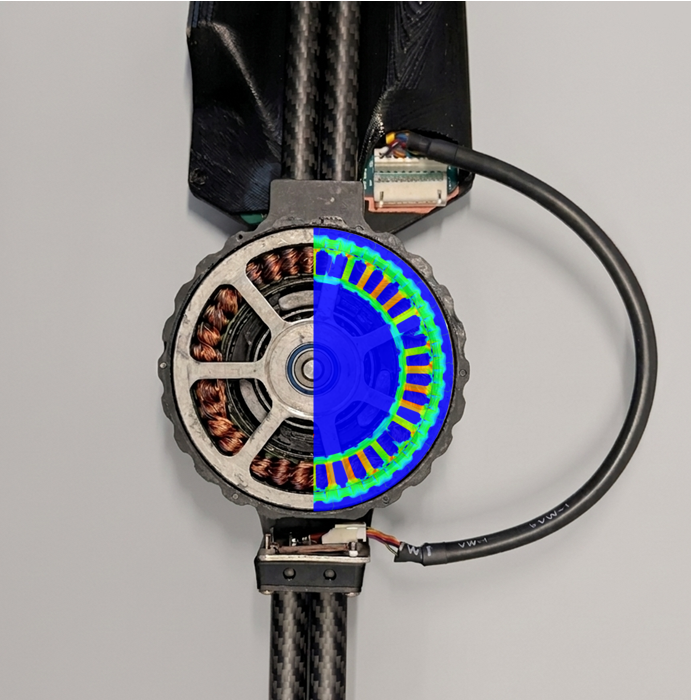
\includegraphics[width=0.5\linewidth]{figures/motor.png}
    \caption{Motor and ANSYS Simulation}
    \label{fig:motor_ansys}
\end{figure}
% --- 3. SCHEDULE AND BUDGETING (10%) ---
\section{Schedule and Budgeting}

\subsection{Project Schedule}
% TODO: Gantt chart review. Milestone tracking. Delay causes.

    Figure \ref{fig:gantt_timeline} below shows the Gantt chart for Exoni's project timeline for developing the mechanical, electrical, and software subsystems.

    \begin{figure}[H]
    \centering
    \resizebox{\textwidth}{!}{% Resizes the chart to fit the page width
    \begin{ganttchart}[
        vgrid={*1{dotted}},
        hgrid,
        x unit=3.5cm,
        y unit title=0.7cm,
        y unit chart=0.7cm,
        title label font=\bfseries\sffamily,
        bar label font=\sffamily,
        bar/.style={fill=blue!20, draw=blue!70, rounded corners=2pt},
        group label font=\bfseries\sffamily,
        group/.style={draw=black, fill=black},
        milestone label font=\sffamily\color{red},
        group label node/.append style={xshift=-0.4cm},
    bar label node/.append style={xshift=-0.2cm}
    ]{1}{4}

    % Milestone Titles
    \gantttitle{Dec 1 -- Jan 4}{1}
    \gantttitle{Jan 4 -- Jan 15}{1}
    \gantttitle{Jan 15 -- Jan 30}{1}
    \gantttitle{Jan 30 -- Feb 15}{1} \\

    % --- Electronics / PCBs ---
    \ganttgroup{Electronics}{1}{4} \\
    \ganttbar{Validate Devboard}{1}{1} \\
    \ganttbar{Design PCBAs}{2}{2} \\
    \ganttbar{Order PCBAs}{3}{3} \\
    \ganttbar{Validate PCBAs}{4}{4} \\

    % --- Hardware / Mechanical ---
    \ganttgroup{Hardware \& Motor}{1}{4} \\
    \ganttbar{PCB Foot, Better Cuffs, Rig}{1}{1} \\
    \ganttbar{Custom BLDC \& QDD}{2}{3} \\
    \ganttbar{Exoskeleton Arms}{2}{3} \\
    \ganttbar{Validate New Motor}{4}{4} \\

    % --- Software / Firmware / ML ---
    \ganttgroup{Software \& Control}{1}{4} \\
    \ganttbar{STM/ESP Code}{1}{2} \\
    \ganttbar{Data Collection \& Training}{2}{2} \\
    \ganttbar{Prediction Development}{3}{3} \\
    \ganttbar{Test Controls}{4}{4}
    \end{ganttchart}
    }
    \caption{Project timeline featuring electrical, mechanical, and software milestones}
    \label{fig:gantt_timeline}
    \end{figure}

\subsection{Budget: Projected vs. Actual Cost}
% TODO: Table comparing expected vs. actual costs.
\begin{table}[H]
\centering
\caption{Projected vs. Actual Budget Breakdown}
\label{tab:budget}
\begin{tabular}{lrr}
\toprule
\textbf{Category / Component} & \textbf{Estimated (\$)} & \textbf{Actual (\$)} \\
\midrule
\multicolumn{3}{l}{\textbf{\textit{Mechanical}}} \\
Actuators (Custom BLDC \& QDD) & 350.00 & 410.00 \\
Structural Materials (Al/Carbon) & 150.00 & 135.00 \\
3D Printing Filament / Resin & 40.00 & 55.00 \\
Hardware (Fasteners, Cuffs) & 60.00 & 75.00 \\
\midrule
\textit{Mechanical Subtotal} & \textit{600.00} & \textit{675.00} \\
\midrule
\multicolumn{3}{l}{\textbf{\textit{Electrical}}} \\
Devboard JLCPCB Fabrication \& Assembly & 80.00 & 120.00 \\
PCBAs JLCPCB Fabrication \& Assembly & 650.00 & 1050.00 \\
Custom Cables & 60.00 & 120.00 \\
\midrule
\textit{Electrical Subtotal} & \textit{790.00} & \textit{1290.00} \\
\midrule
\textbf{Total} & \textbf{1390.00} & \textbf{1965.00} \\
\bottomrule
\end{tabular}
\end{table}

% --- 4. CONCLUSIONS AND RECOMMENDATIONS (10%) ---
\section{Conclusions and Recommendations}

\subsection{Conclusions}

Exoni demonstrates that a custom-designed powered knee exoskeleton meeting the conflicting constraints of high torque density, low backdrive resistance, passive thermal safety, and minimal mass is achievable within a capstone project scope. The simulation-driven design methodology --- progressing from electromagnetic FEA to motor thermal CHT to battery thermal CHT --- was essential: none of the three key design decisions (stator frame, rotor configuration, battery configuration) could have been made correctly by intuition alone.

The final system meets all five design constraints. Most notably, the Halbach rotor configuration reduced backdrive torque by $6\times$ relative to an iron-backed default while simultaneously reducing rotor weight by 2.88$\times$, and the battery thermal analysis enabled a configuration change from 6s2p to 8s1p, saving approximately 300~g. The second motor iteration achieved torque constant within 5\% of simulation, validating the electromagnetic model after accounting for 2D simulation limitations in the first iteration.

The three custom PCBAs were successfully designed and validated, resulting in safe operation with the custom battery pack. The custom firmware successfully brought up all subsystems: ADC current-offset calibration, AS5048A encoder reads at 1~kHz, dual IMU reads at 200~Hz, and closed-loop FOC commutation of the custom BLDC motor. In closed-loop mode, $i_d$ converged to near zero and $i_q$ tracked its reference with low steady-state error, confirming correct encoder-to-electrical-frame alignment and well-tuned PI current controllers. The binary telemetry stream provided a continuous 200~Hz data feed for validation and future system integration.
\begin{figure}
    \centering
    \includegraphics[width=0.5\linewidth]{figures/final.jpg}
    \caption{Final Result -- In Deployment}
    \label{fig:final_result}
\end{figure}
\subsection{Recommendations for Future Work}

Several directions are identified for future development of the Exoni platform.

On the mechanical side, further mass reduction through carbon fibre structural components and a higher gear ratio would improve torque density while reducing overall system weight below 1.5~kg.

On the firmware and control side, the most impactful near-term improvement would be the implementation of sensorless FOC using back-EMF observers, eliminating the encoder cable and connector as a potential failure point in outdoor use. The current impedance control law uses fixed stiffness and damping parameters; a phase-adaptive impedance controller --- varying $K$ and $D$ based on detected gait phase --- would allow the exoskeleton to provide more targeted assistance during stance push-off and swing-phase knee flexion. Additionally, the current PI current controller gains were tuned empirically; a model-based auto-tuning procedure using the identified motor electrical parameters ($R$, $L$) would make commissioning faster and more repeatable for future hardware iterations. Finally, extending the firmware to support bilateral operation (two motor drives communicating over a low-latency bus) and adding a real-time safety monitor for the impedance output bounds would be necessary prerequisites for clinical validation trials.


% --- 5. TEAMWORK EFFORT (5%) ---
\section{Teamwork Effort}
% TODO: 1--2 pages. Per-member contributions across mechanical, electrical, and firmware domains
Egor Gorelyy handled all mechanical work behind Exoni.
 Tasks included:
 \begin{itemize}
        \item Requirement gathering, design, simulation of a fully custom motor.
        \item Full fabrication of a custom motor.
        \item Motor testing and characterization.
        \item Ergonomic cuff design and testing.
        \item Basically everything else on the mechanical side.
        \item Working with Taim (electrical) to fit custom cables, PCBAs, and more to ensure integration
    \end{itemize}
Taim Al-Dabbagh handled all electrical work behind Exoni. Tasks included:
    \begin{itemize}
        \item Architecting the initial electrical system for minimum viable product
        \item Designing and assembling the devboard
        \item Board-bring up for the devboard
        \item Reiteration and design of 3 PCBAs
        \item Working with Egor (mechanical) to fit custom cables, PCBAs, and more to ensure integration
        \item Worked with manufacturers for PCBAs and custom cables
        \item Board bring-up and validation of PCBAs and cables
        \item Supporting team with other small tasks (motor assembly for example)
    \end{itemize}
Hasan Khan handled all firmware and half of embedded software work behind Exoni. Tasks included:
\begin{itemize}
\item Architecting dual-task FreeRTOS firmware for motor and control loops.
\item Implementing the full Field Oriented Control (FOC) pipeline and SVPWM.
\item Developing SPI drivers for magnetic encoders and dual IMUs.
\item Creating encoder calibration and electrical angle alignment routines.
\item Designing the motor control state machine and open-loop soft-start.
\item Implementing the impedance control loop for compliant knee assistance.
\item Developing binary telemetry for data transmission.
\item Commissioning and validating firmware on custom hardware.
\item Working with Taim (electrical) to debug hardware/firmware integration.
\end{itemize}

Nolen Zhao handled the higher level controls algorithm construction and low latency pefromance software. Tasks included: 
\begin{itemize}
    \item Architecting multi-layer control pipeline for low-latency communication.
    \item Converting raw sensor reads into torque target and current control for input to FOC.
    \item Profiling performance of critical path for control loop to increase resolution and make system faster to respond.
    \item Developing telemetry interface for live IMU, torque, and current monitoring through WiFi and bluetooth.
    \item Develop impedance control based on reference gait cycle and spring-damper simulation.
    \item Cleaned motion-capture (MOCAP) to drop corrupted samples and outliers.
    \item Trained and fine tuned random forest classification ML model on gathered MOCAP gait data.
\end{itemize}


% --- 8. REPORT QUALITY & CLARITY (References) ---
\clearpage
\bibliographystyle{IEEEtran}
\bibliography{references}
\addcontentsline{toc}{section}{References}


% --- 7. SUPPORTING DOCUMENTS & ENGINEERING DRAWINGS (10%) ---
\clearpage
\appendix

\section{Detailed Information and Calculations}
% Full Ansys Maxwell electromagnetic calculation data, SimScale thermal simulation data, battery capacity math, FOC tuning math, etc.

\section{As-Built Engineering Drawings}
Alas, there is no documentation on this matter.

\begin{figure}
    \centering
    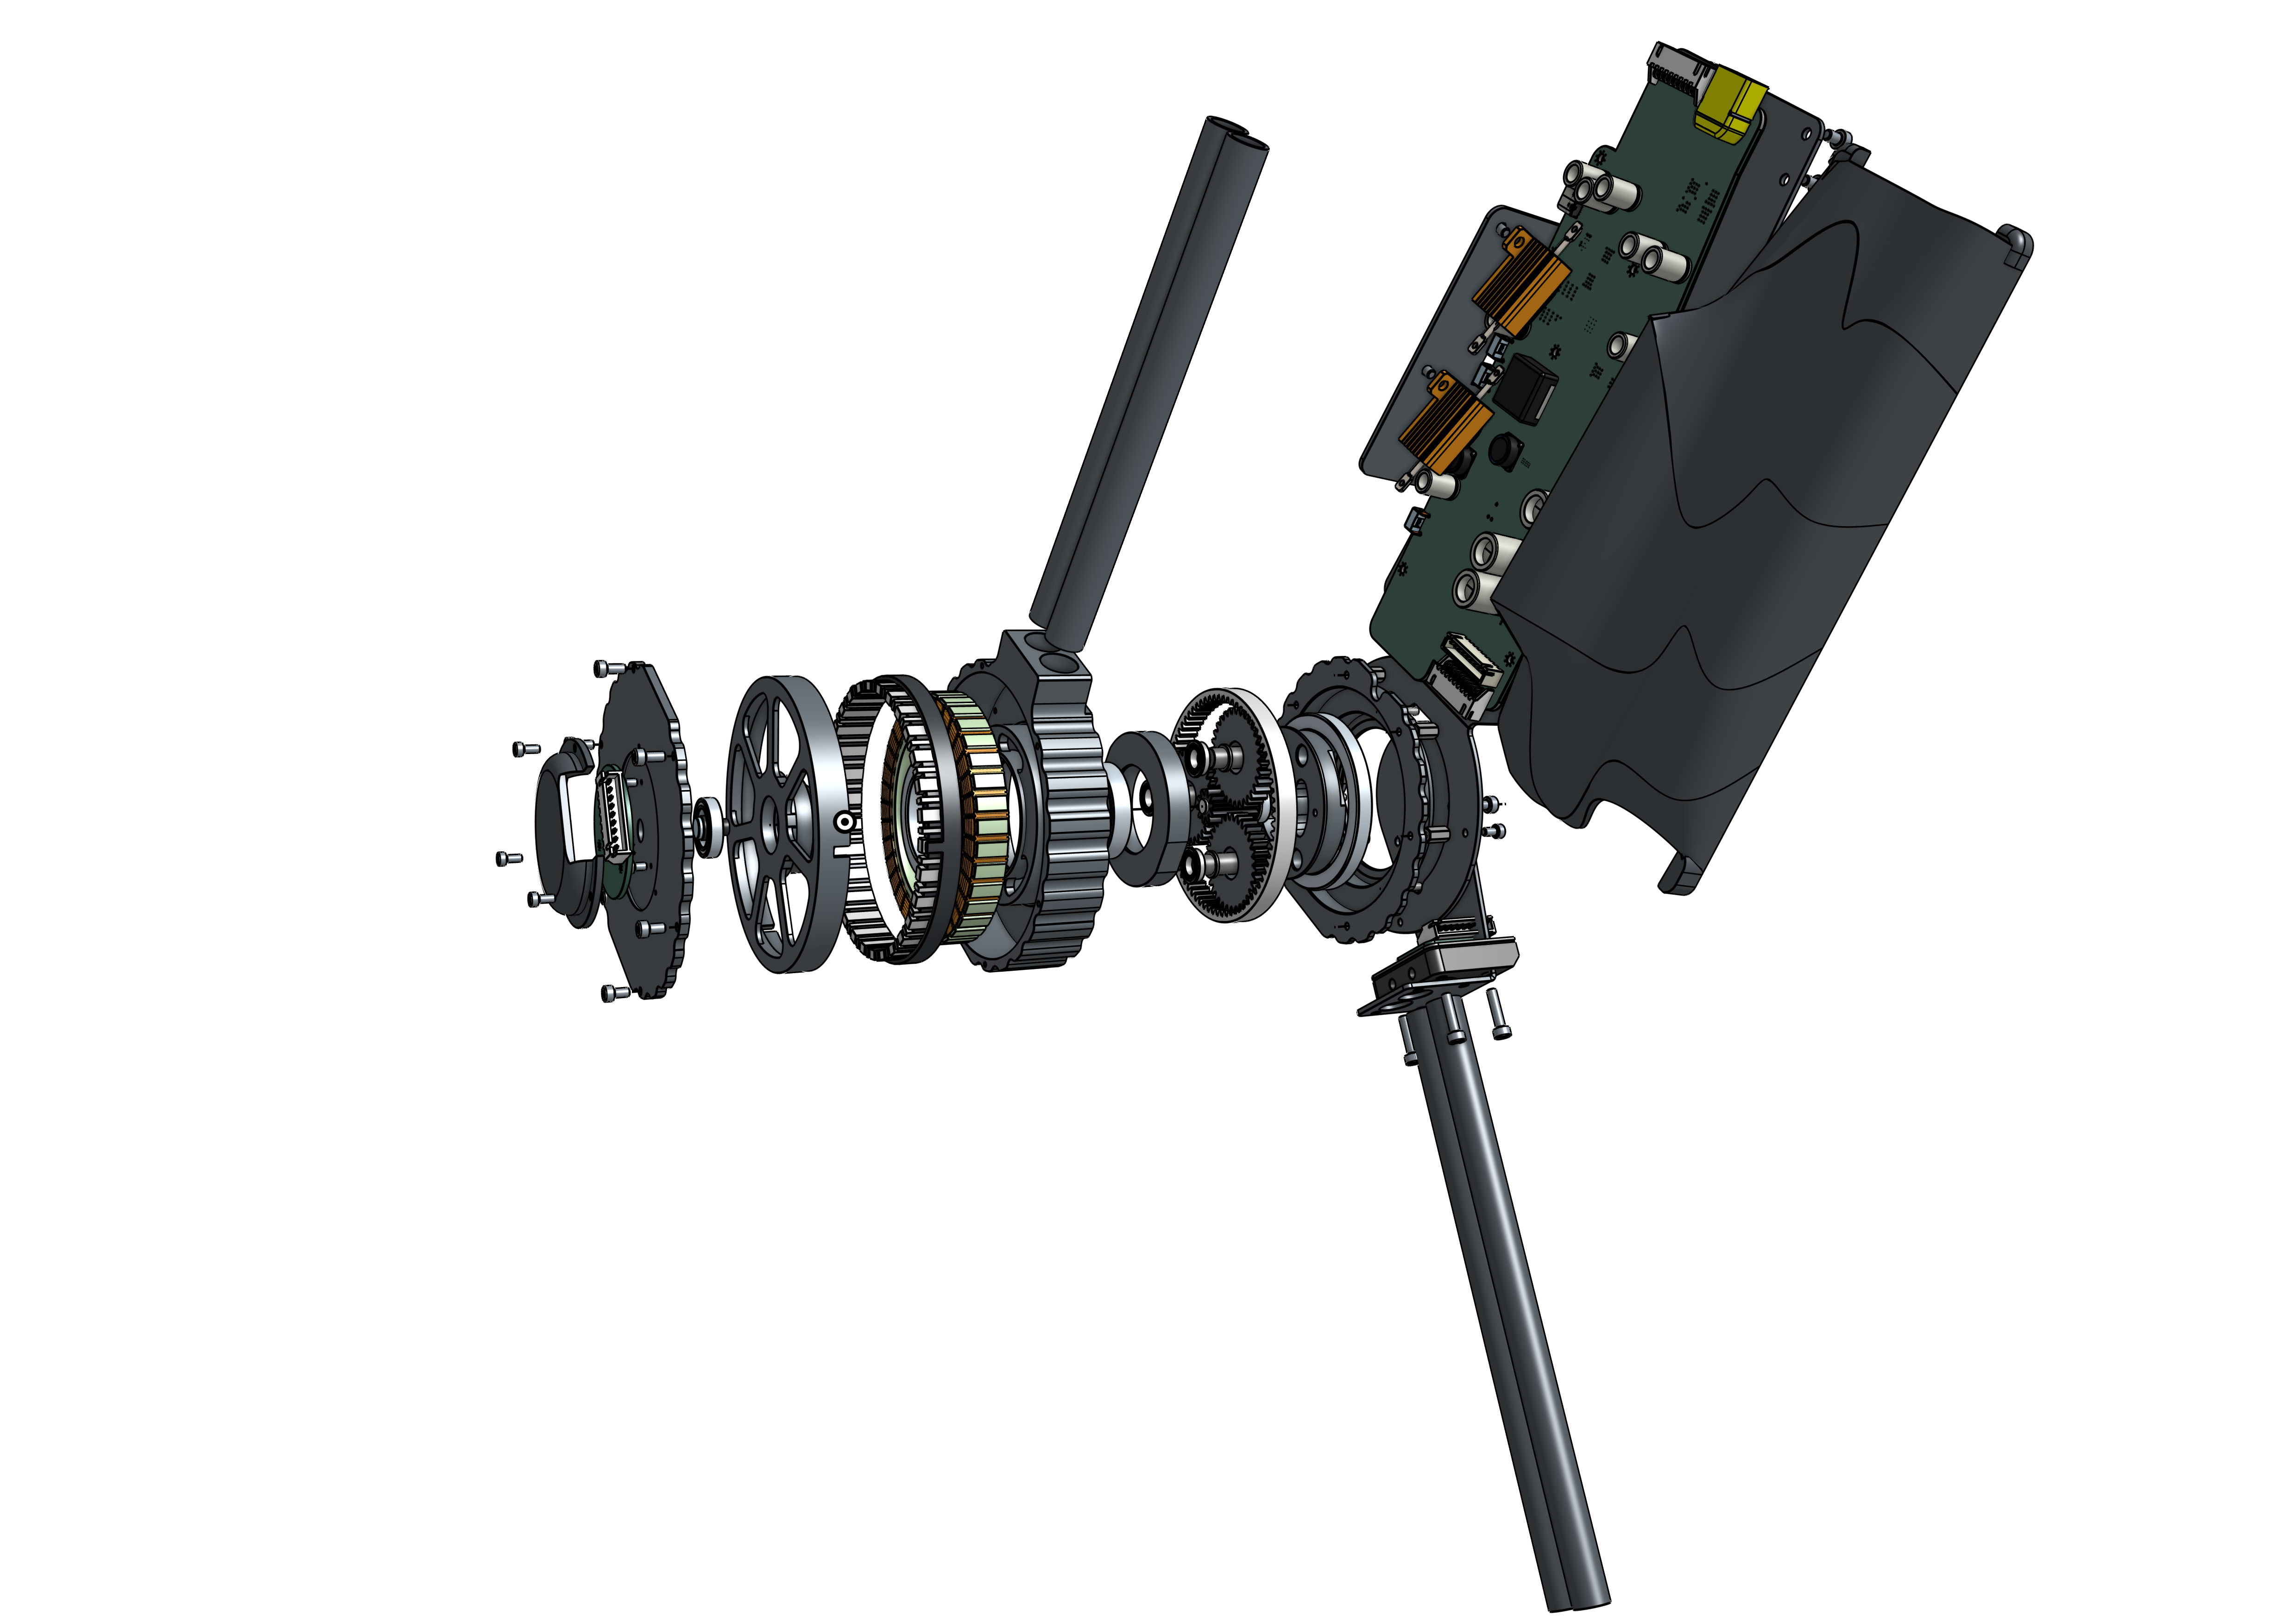
\includegraphics[width=0.5\linewidth]{figures/blown up.png}
    \caption{Blown Up System Assembly}
    \label{fig:system_exploded}
\end{figure}


\end{document}
